\begin{frame}{Seat Planning with Social Distancing}
  \begin{itemize}  
    \item Group type $\mathcal{M} = \{1, \ldots, M\}$.
    \item Row $\mathcal{N} = \{1, \ldots, N\}$.
    \item The number of seats in row $j$: $L_j^{0}, j \in \mathcal{N}$.
    \item The social distancing: $\delta$ seat(s).
    \item[-] $n_i = i + \delta$: the size of group type $i$ for each $i \in \mathcal{M}$.
    \item[-] $L_j = L_j^{0} + \delta$: the length of row $j$ for each $j \in \mathcal{N}$.
    \end{itemize}
    
    \begin{figure}[ht]
      \centering
      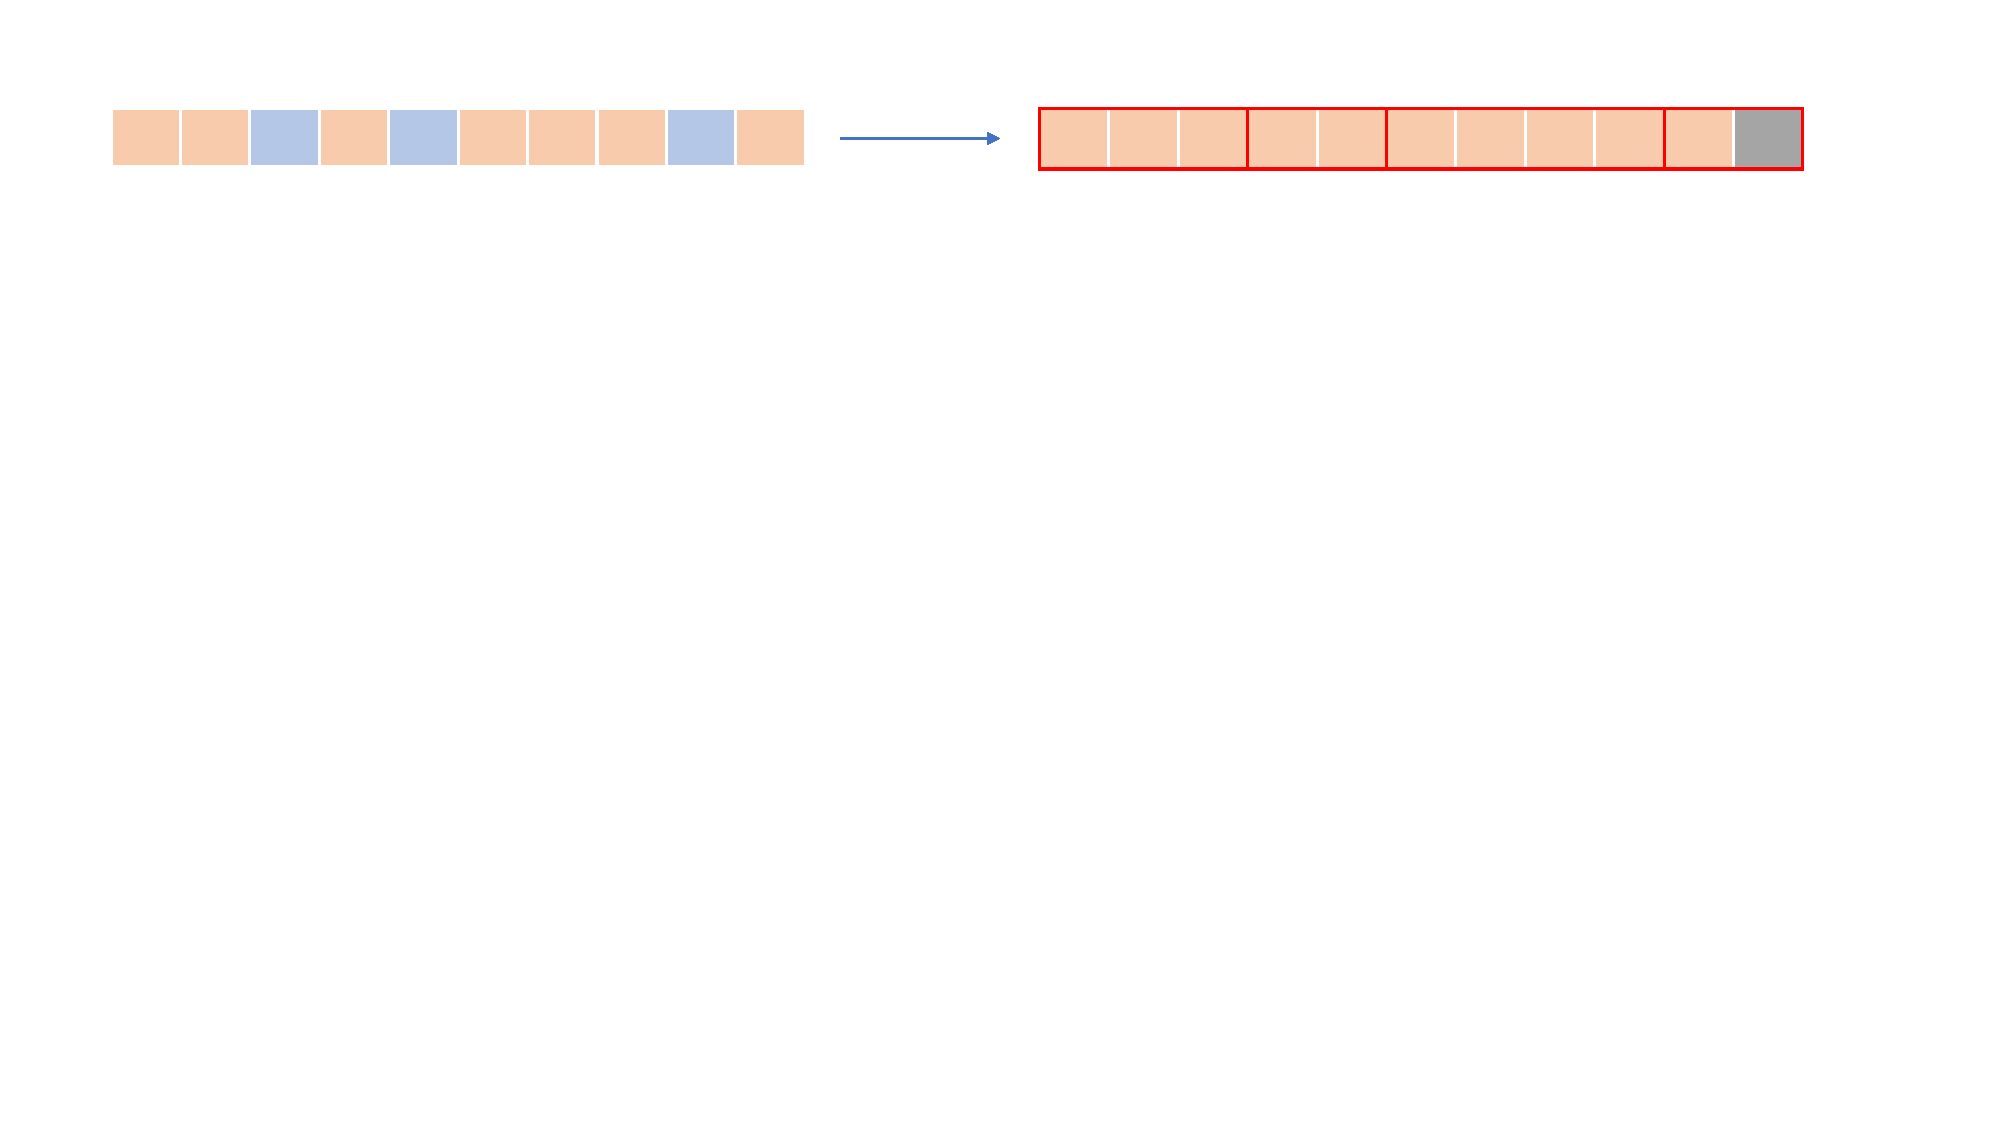
\includegraphics[width = 0.8\textwidth]{./images/dummy_seat.pdf}
      \caption{Problem Conversion with One Seat as Social Distancing}
  \end{figure}
  \end{frame}

  \begin{frame}{Pattern}
    \begin{itemize}
      \item Pattern: $\bm{h} = (h_1, \ldots, h_M)$, the seat planning for one row, where $h_i$ is the number of group type $i$.

      - The number of people accommodated: $|\bm{h}| = \sum_{i =1}^{M} i h_i$.
    \end{itemize}
    
    \begin{figure}[ht]
      \centering
      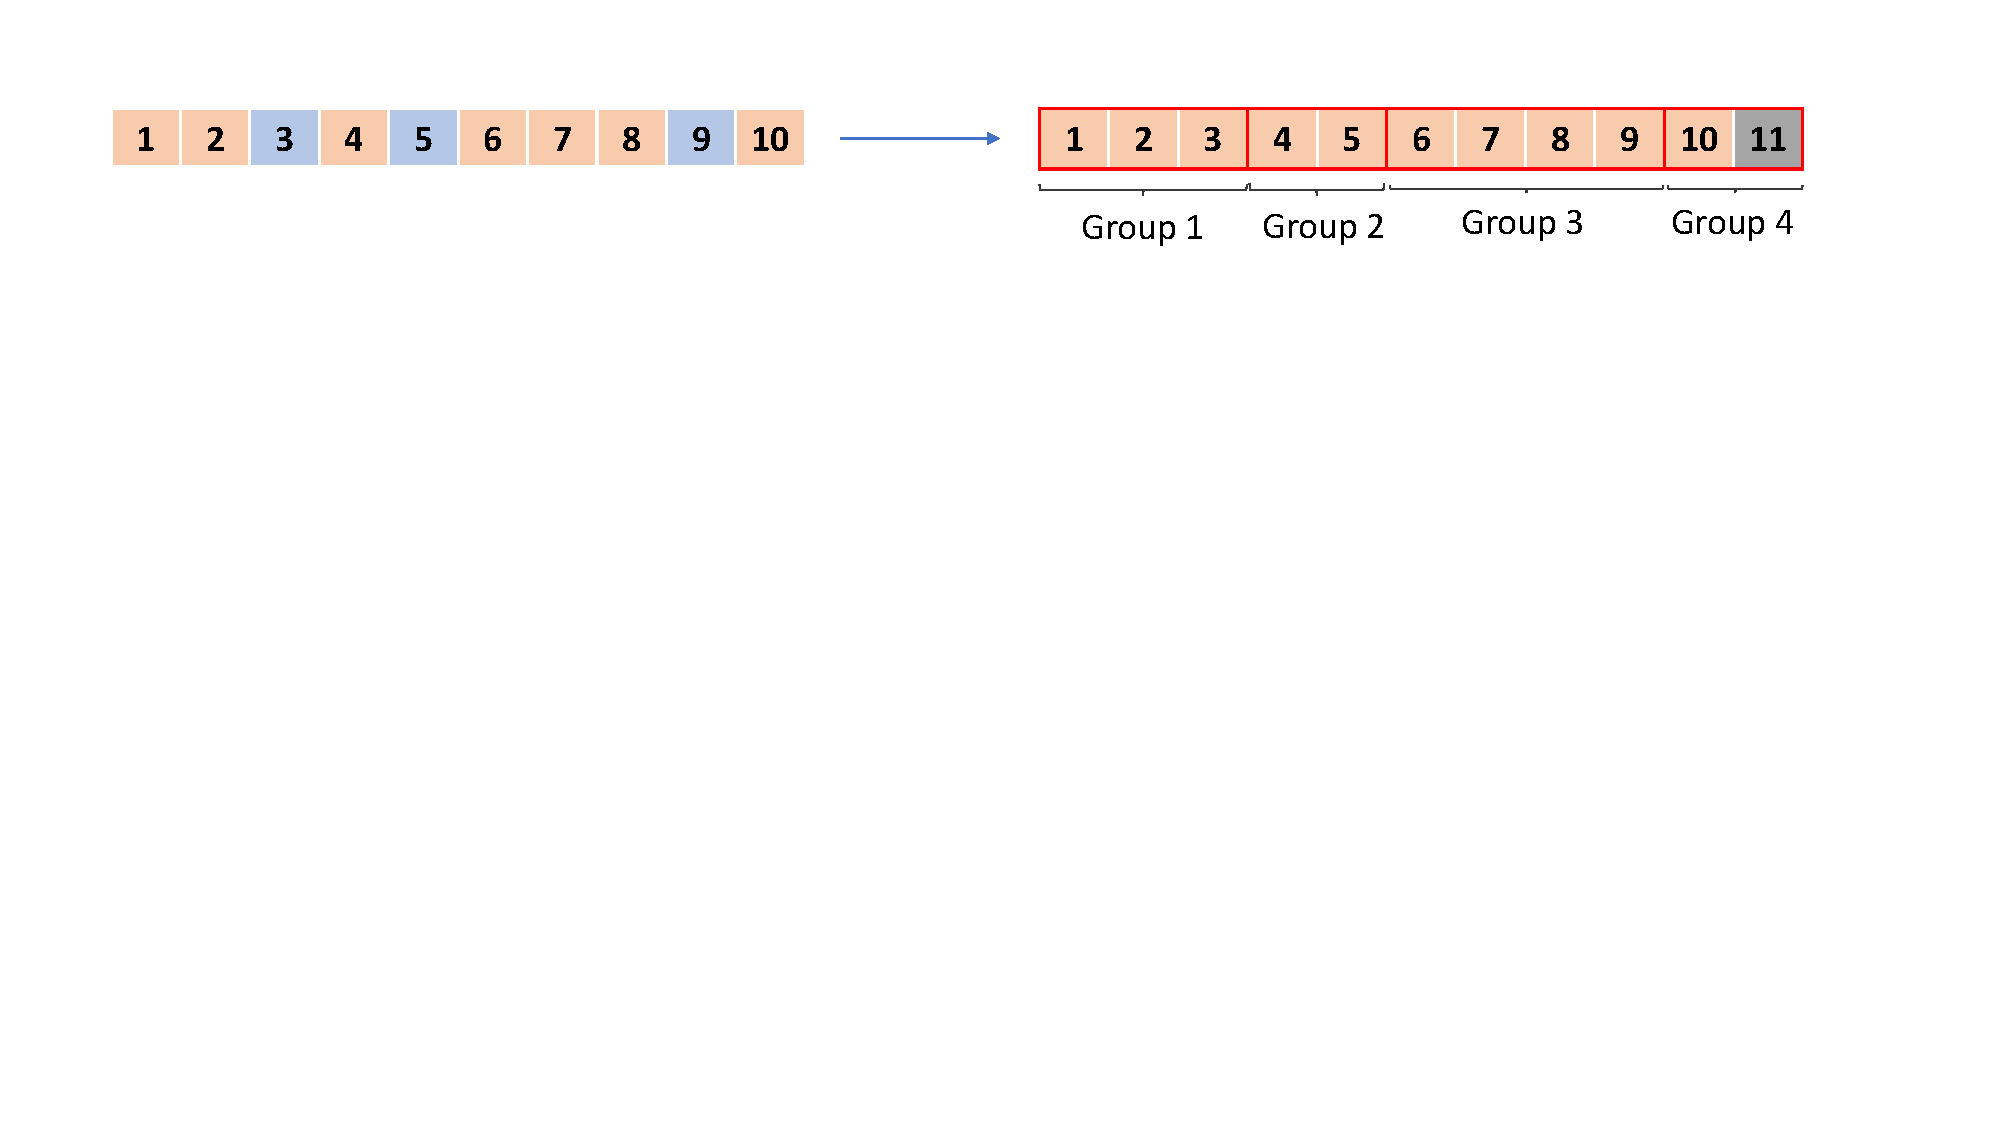
\includegraphics[width = 0.8\textwidth]{./images/conversion.pdf}
    \end{figure}
    \centering
    $L = 11$, $\delta =1$, $M =4$, $n_1 = 2, n_2 = 3, n_3 = 4, n_4 = 5$. 

    $\bm{h} = (2, 1, 1, 0)$, $|\bm{h}| = 7$.
  \end{frame}

  \begin{frame}{Largest and Full Patterns}
    Suppose the length of the row is $L$.
    \begin{itemize}
      \item[-] $\bm{h}$ is a feasible pattern if $\sum_{i=1}^{M} n_i h_i \leq L$.
      \item[-] $\bm{h}$ is a {\color{red}largest} pattern if $|\bm{h}| \geq |\bm{h}^{\prime}|$ for any feasible $\bm{h}^{\prime}$.
      
      $|\bm{h}| = qM + \max\{r-\delta, 0\}$, where $q = \lfloor L/n_M \rfloor$, $r \equiv L \bmod n_M$.
      \item[-] $\bm{h}$ is a {\color{red}full} pattern if $\sum_{i=1}^{M} n_i h_i = L$.  
    \end{itemize}

     {\color{green} Example}: 
      
      $\delta = 1$, $M =4$, $L = 21$.
      
      Largest patterns: $h_1 = (0, 0, 0, 4)$, $h_2 = (0, 0, 4, 1)$, $h_3 = (0, 2, 0, 3)$.

      Largest may not be full: $h_1 = (0, 0, 0, 4)$. {\color{red} $\quad$ $\sum_{i=1}^{M} n_i h_i \neq L$}

      Full may not be largest: $h_4 = (1, 1, 4, 0)$. {\color{red} $|h_4| = 15 < 16 = |h_1|$}

      \begin{figure}[ht]
        \centering
        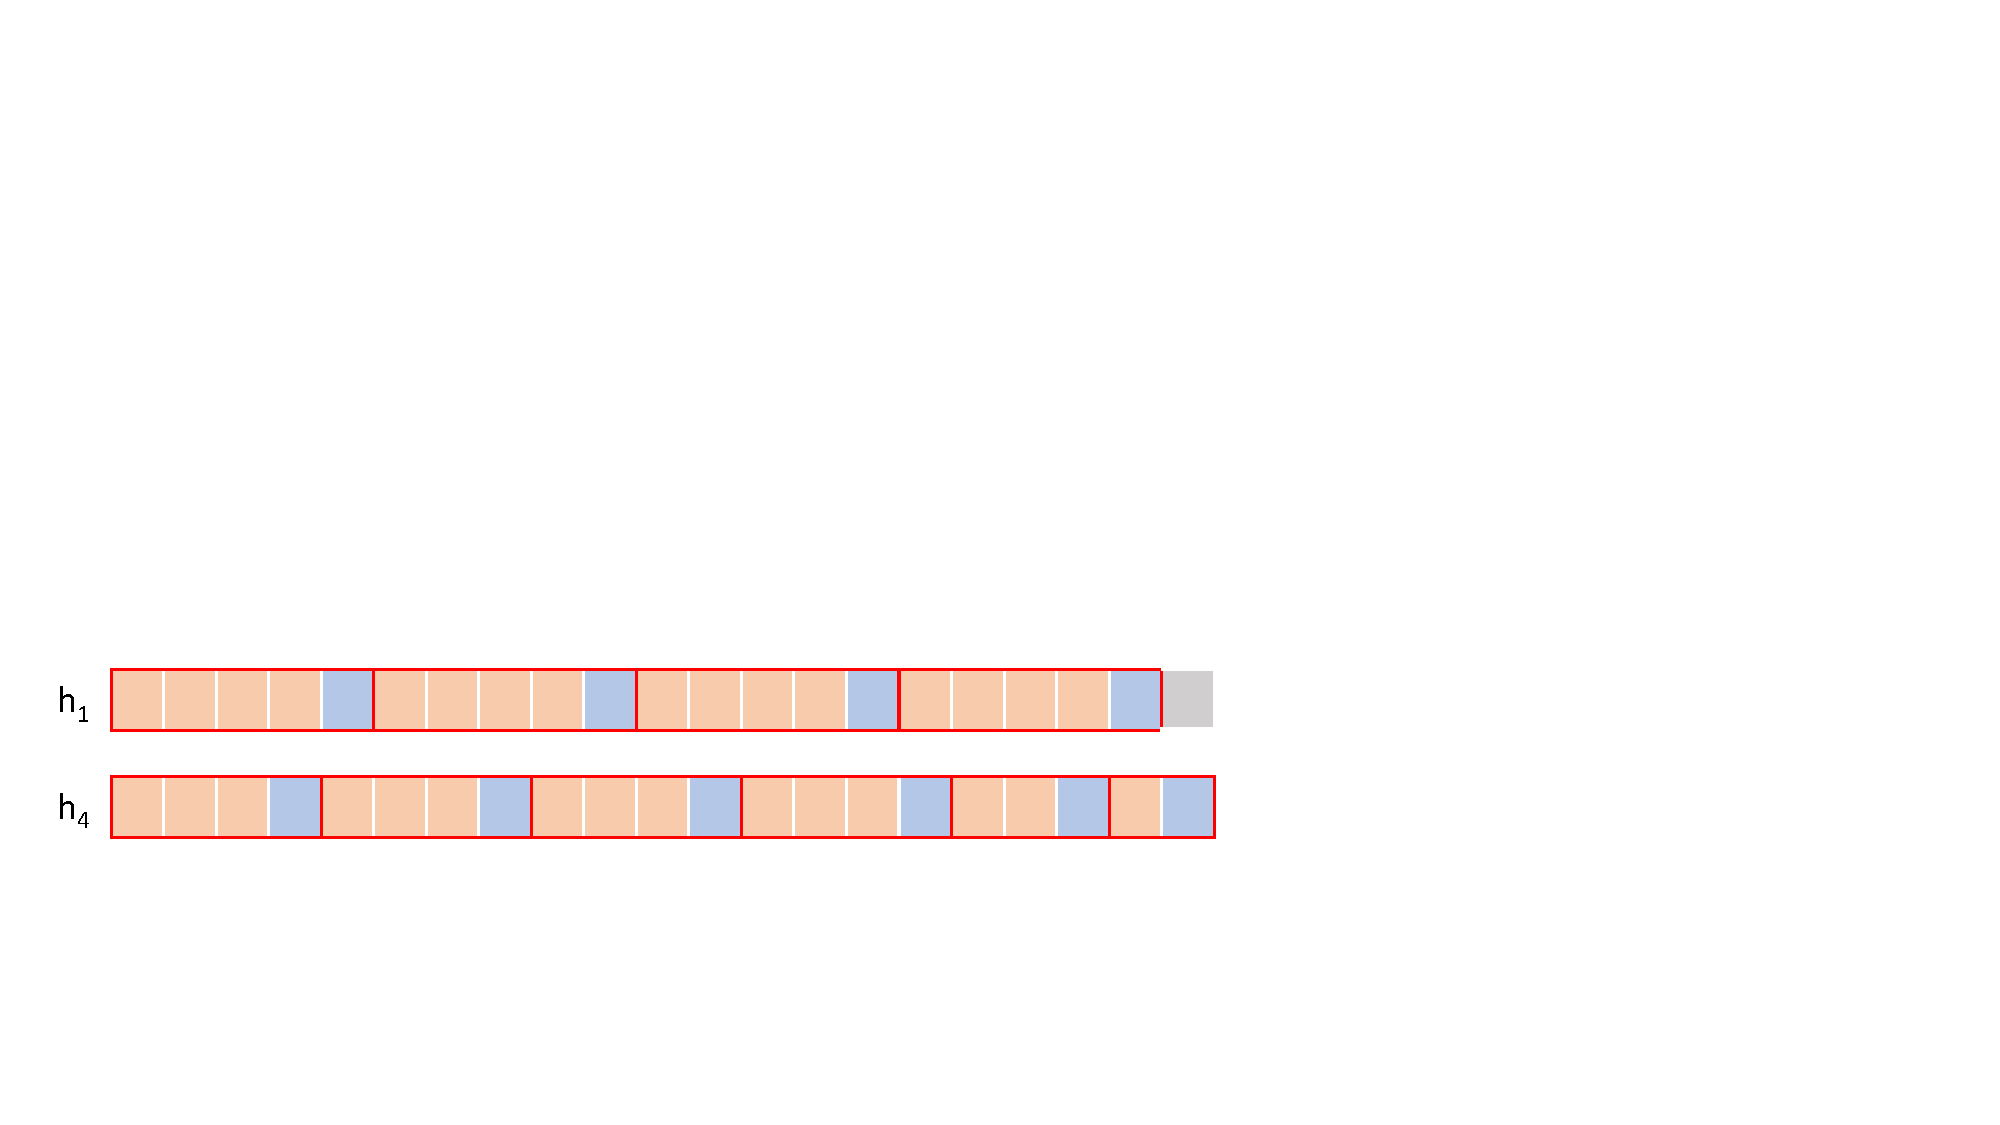
\includegraphics[width = 0.8\textwidth]{./images/full_largest.pdf}
      \end{figure}
  \end{frame}